%%% Local Variables:
%%% mode: latex
%%% TeX-master: "../doc"
%%% coding: utf-8
%%% End:
% !TEX TS-program = pdflatexmk
% !TEX encoding = UTF-8 Unicode
% !TEX root = ../doc.tex

This section describes the approaches and methods applied in the project. These consist of the general approach, the organisation methodology chosen, the use of Git version control and the project schedule set up at the beginning of the project.

\section{Realization of project}
\subsection{Proof that approach of bachelor thesis is applicable}
The first step as to realisation of this project was to prove whether the approach given by the bachelor thesis on which the project is founded is applicable. Since neither one of us has ever worked with Blazor or the related technologies used in the bachelor thesis, the consideration of the software prototype was of particular importance. Both the prototype (see chapter tbd) and the concept of mapping Toggl Track data to ATP data (see chapter tbd) have been investigated in detail. This was done using the documentation of the bachelor thesis, the software code of the prototype and the Blazor online documentation. Thus a fundamental understanding of the approach has been gained. Moreover, our .NET teacher, Mr. Rege, has agreed to provide technological support for Blazor and related technologies. In the light of all this, the approach has been considered applicable and therefore served as basis for the realisation of this project.

\subsection{Implementation of mapping concept}
To be able to actually handle data in the application, the mapping concept designed in the bachelor thesis (see chapter \ref{Mapping concept}) had to be implemented. The implementation generally follows the mapping concept apart from a few class attributes which were deleted since they were not considered to be needed. The data is made persistent for the current browser session by being stored using Local Storage (see chapter tbd) and can be accessed from the application via a data manager object which is unique for every browser session.

\subsection{Research of alternative chart display possibilities}
Since the comparison between planned and tracked time should be displayed graphically, there had to be a possibility to display data using charts. The approach suggested in the bachelor thesis was to use the JavaScript library Charts.js and call it directly out of the application. However, this was not considered to be the best way to display charts since JavaScript code had to be added manually and called using code injection. Therefore, we decided to dedicate some time to investigate more elegant alternatives. The following packages offer functionality to create charts in Blazor without having to write JavaScript code:
\begin{itemize}
	\item Blazorise \cite{blazorise-url}
	\item ChartsJs.Blazor \cite{chartsjs.blazor-url}
	\item Plotly.Blazor \cite{plotly-url}
	\item Radzen \cite{radzen-url}
\end{itemize}
All four packages were tested by trying to include a sample chart into the application. Apart from ChartsJs.Blazor, which happened to have some installation issues, all packages could easily be installed and integrated. The following pictures show sample charts generated by the different packages being displayed in the ATP.

\begin{figure}[H]
	\centering
	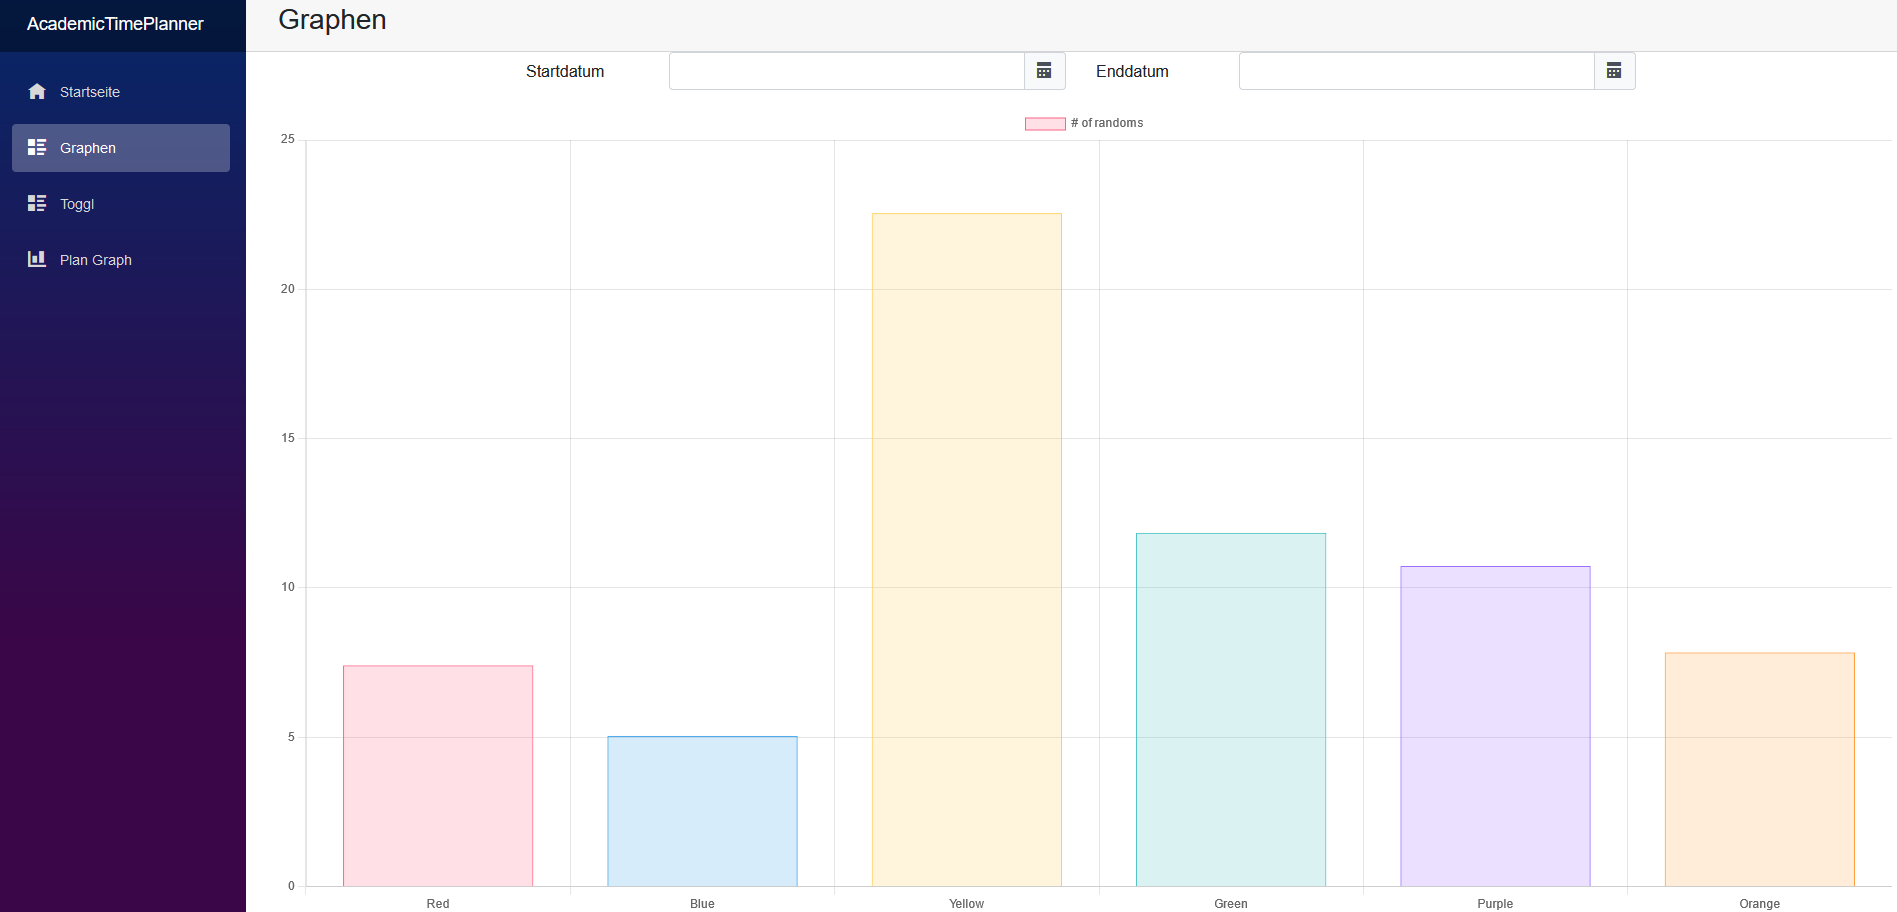
\includegraphics[width=1.0\columnwidth]{blazorise-charts}
	\caption{Blazorise sample charts on the ATP charts page}
	\label{figure5}
\end{figure}

\begin{figure}[H]
	\centering
	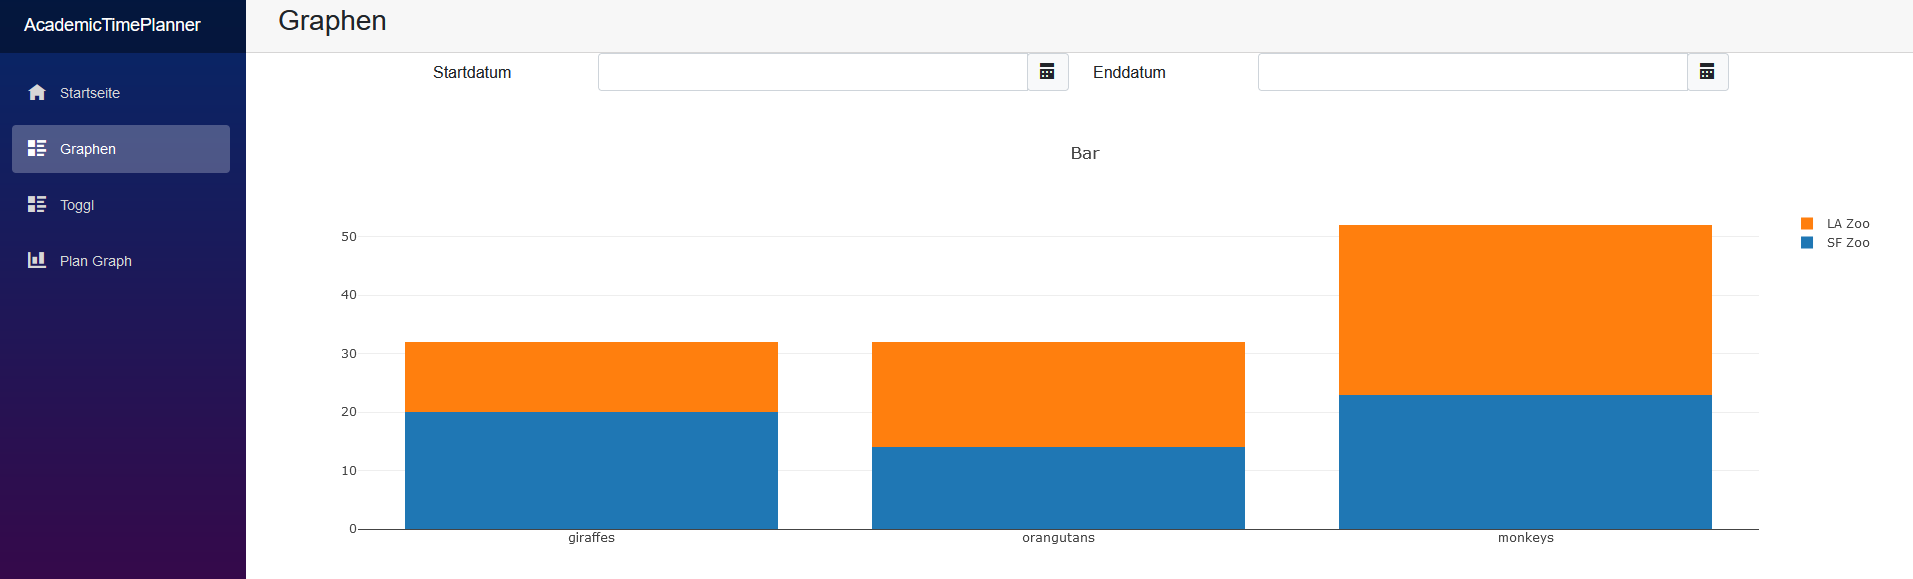
\includegraphics[width=1.0\columnwidth]{plotly-charts}
	\caption{Plotly.Blazor sample charts on the ATP charts page}
	\label{figure6}
\end{figure}

\begin{figure}[H]
	\centering
	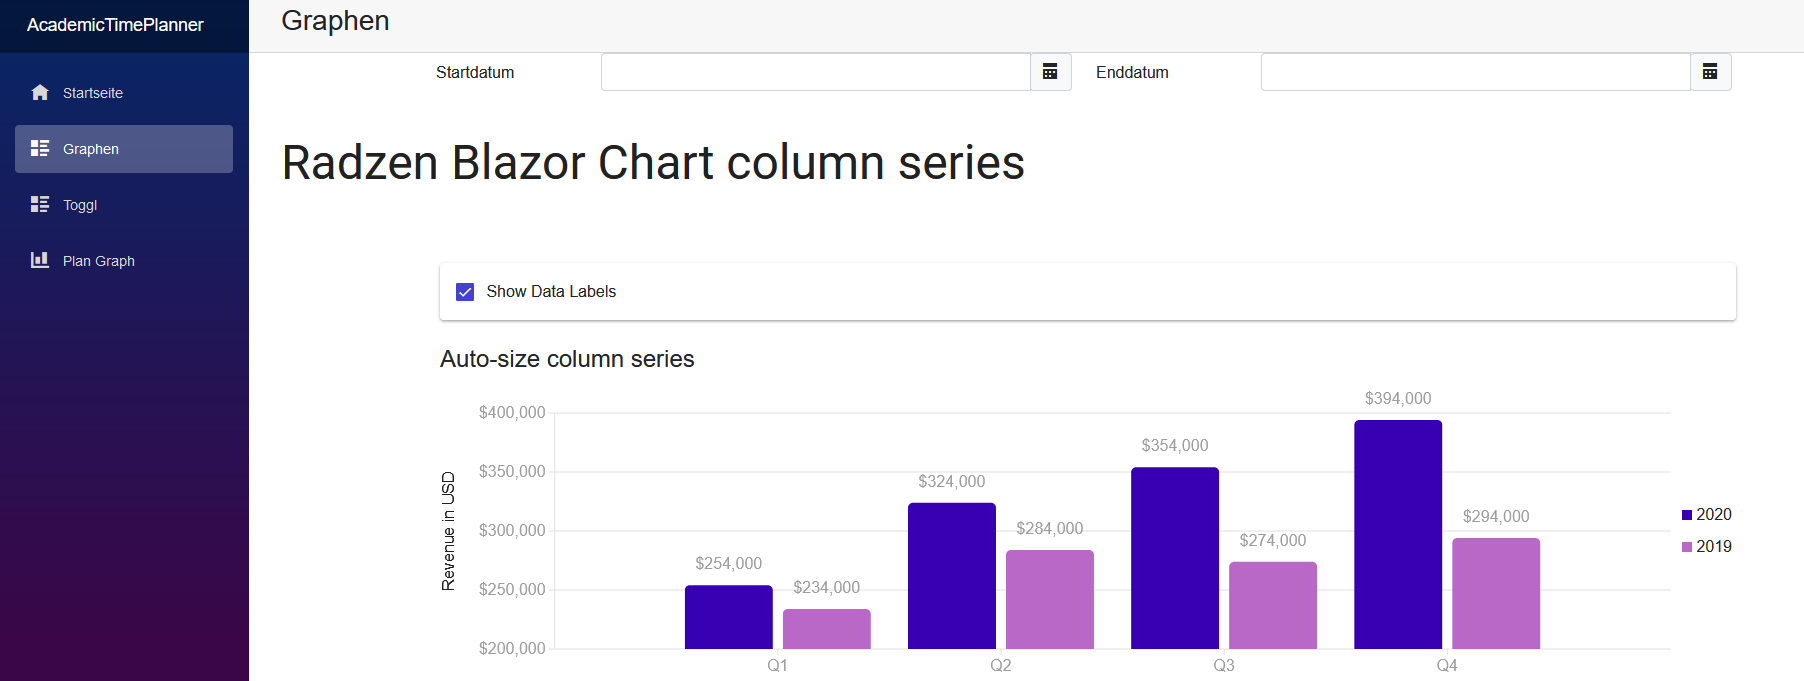
\includegraphics[width=1.0\columnwidth]{radzen-charts}
	\caption{Radzen sample charts on the ATP charts page}
	\label{figure7}
\end{figure}

\subsection{Test projects}
To correctly simulate a working environment test projects were created. These projects include a toggl project with the same characteristics as a real project imported from TogglTrack. This allowed to simulate the situation without the need of a real project from TogglTrack. A further test project was a JSON file which simulated a real save state of a plan project. This allowed to test the loading of a saved plan project as well as the use of said project internally for other methods like the display of the discrepancy of the plan project and the current state in the toggl project. The combination of these two projects allowed the whole application to run without the need for real data while still displaying reasonable values for the user.

\section{Organization methodology}
For this project a reduced and modified version of SCRUM \cite{scrum_url} was chosen. The modifications include reducing the daily SCRUM meetings to two to three meetings a week, as we did not work on the project full time. One of these meetings was also attended by our project advisor Mr. Feisthammel. This meeting was usually held on Tuesday morning. There, a short progress report as well as the next weekly goals were discussed. Milestones as described in chapter \ref{Time management} have been defined. They roughly correspond with the two-week sprint plan. An additional reduction is the absence of a sprint review as we do something similar in the weekly meetings described above. The point system as well as the burn down chart were also dropped.

\section{Git}
For appropriate software code management, the Git version control system and the online service GitHub (see chapter \ref{Version control}) have been used. The software code was stored in a GitHub repository named "academic-time-planner". The main branch always represented the current state of the software, containing all tested and approved features. New features were implemented via feature branches named according to the pattern "feature/name-of-member/feature-description". The software tests were executed automatically via GitHub Actions (see chapter \ref{GitHub Actions}) on every push to a feature branch. The result of the automated tests were taken into account in the feature pull requests. The documentation was kept in the same repository and was treated like the software code in the sense that additions and changes had to be reviewed and approved via pull requests, as was the software code. Documentation branches were named after the "documentation/name-of-member/section-description". Tasks were managed via GitHub issues (see chapter \ref{GitHub Issues}).

\section{Time management} \label{Time management}
Four milestones were proposed at the beginning of the project. They were taken from the project outline and include three programming milestones and one documentation milestone. The first one was the implementation of the overview of difference between plan and tracking, followed by the application status display. The final programming milestone was composed of the import and export as well as the creation of plan projects. After this the documentation had to be finalized. These milestones were meant as a guideline to see if the progress was adequate or if we had to rethink our approach. Those milestones were created and managed in GitHub (see chapter \ref{GitHub}). 



